In Section~\ref{sec:metric_spaces} we show multiple ways of endowing the mapping space with a distance metric.
A common method for defining a metric in a \ac{NoC}-based system is to count the number of hops between two processors~\cite{singh2010communication,schwarzer2017symmetry}.
Indeed, this is the same as the $L_1$ (Manhattan) distance on the topology graph of the architecture.
A natural idea that arises from this is to search for \emph{compact} mappings\index{compact mappings}, i.e. mappings that take a (geometrically) small area in the chip.


\begin{figure*}[th]
	\centering
	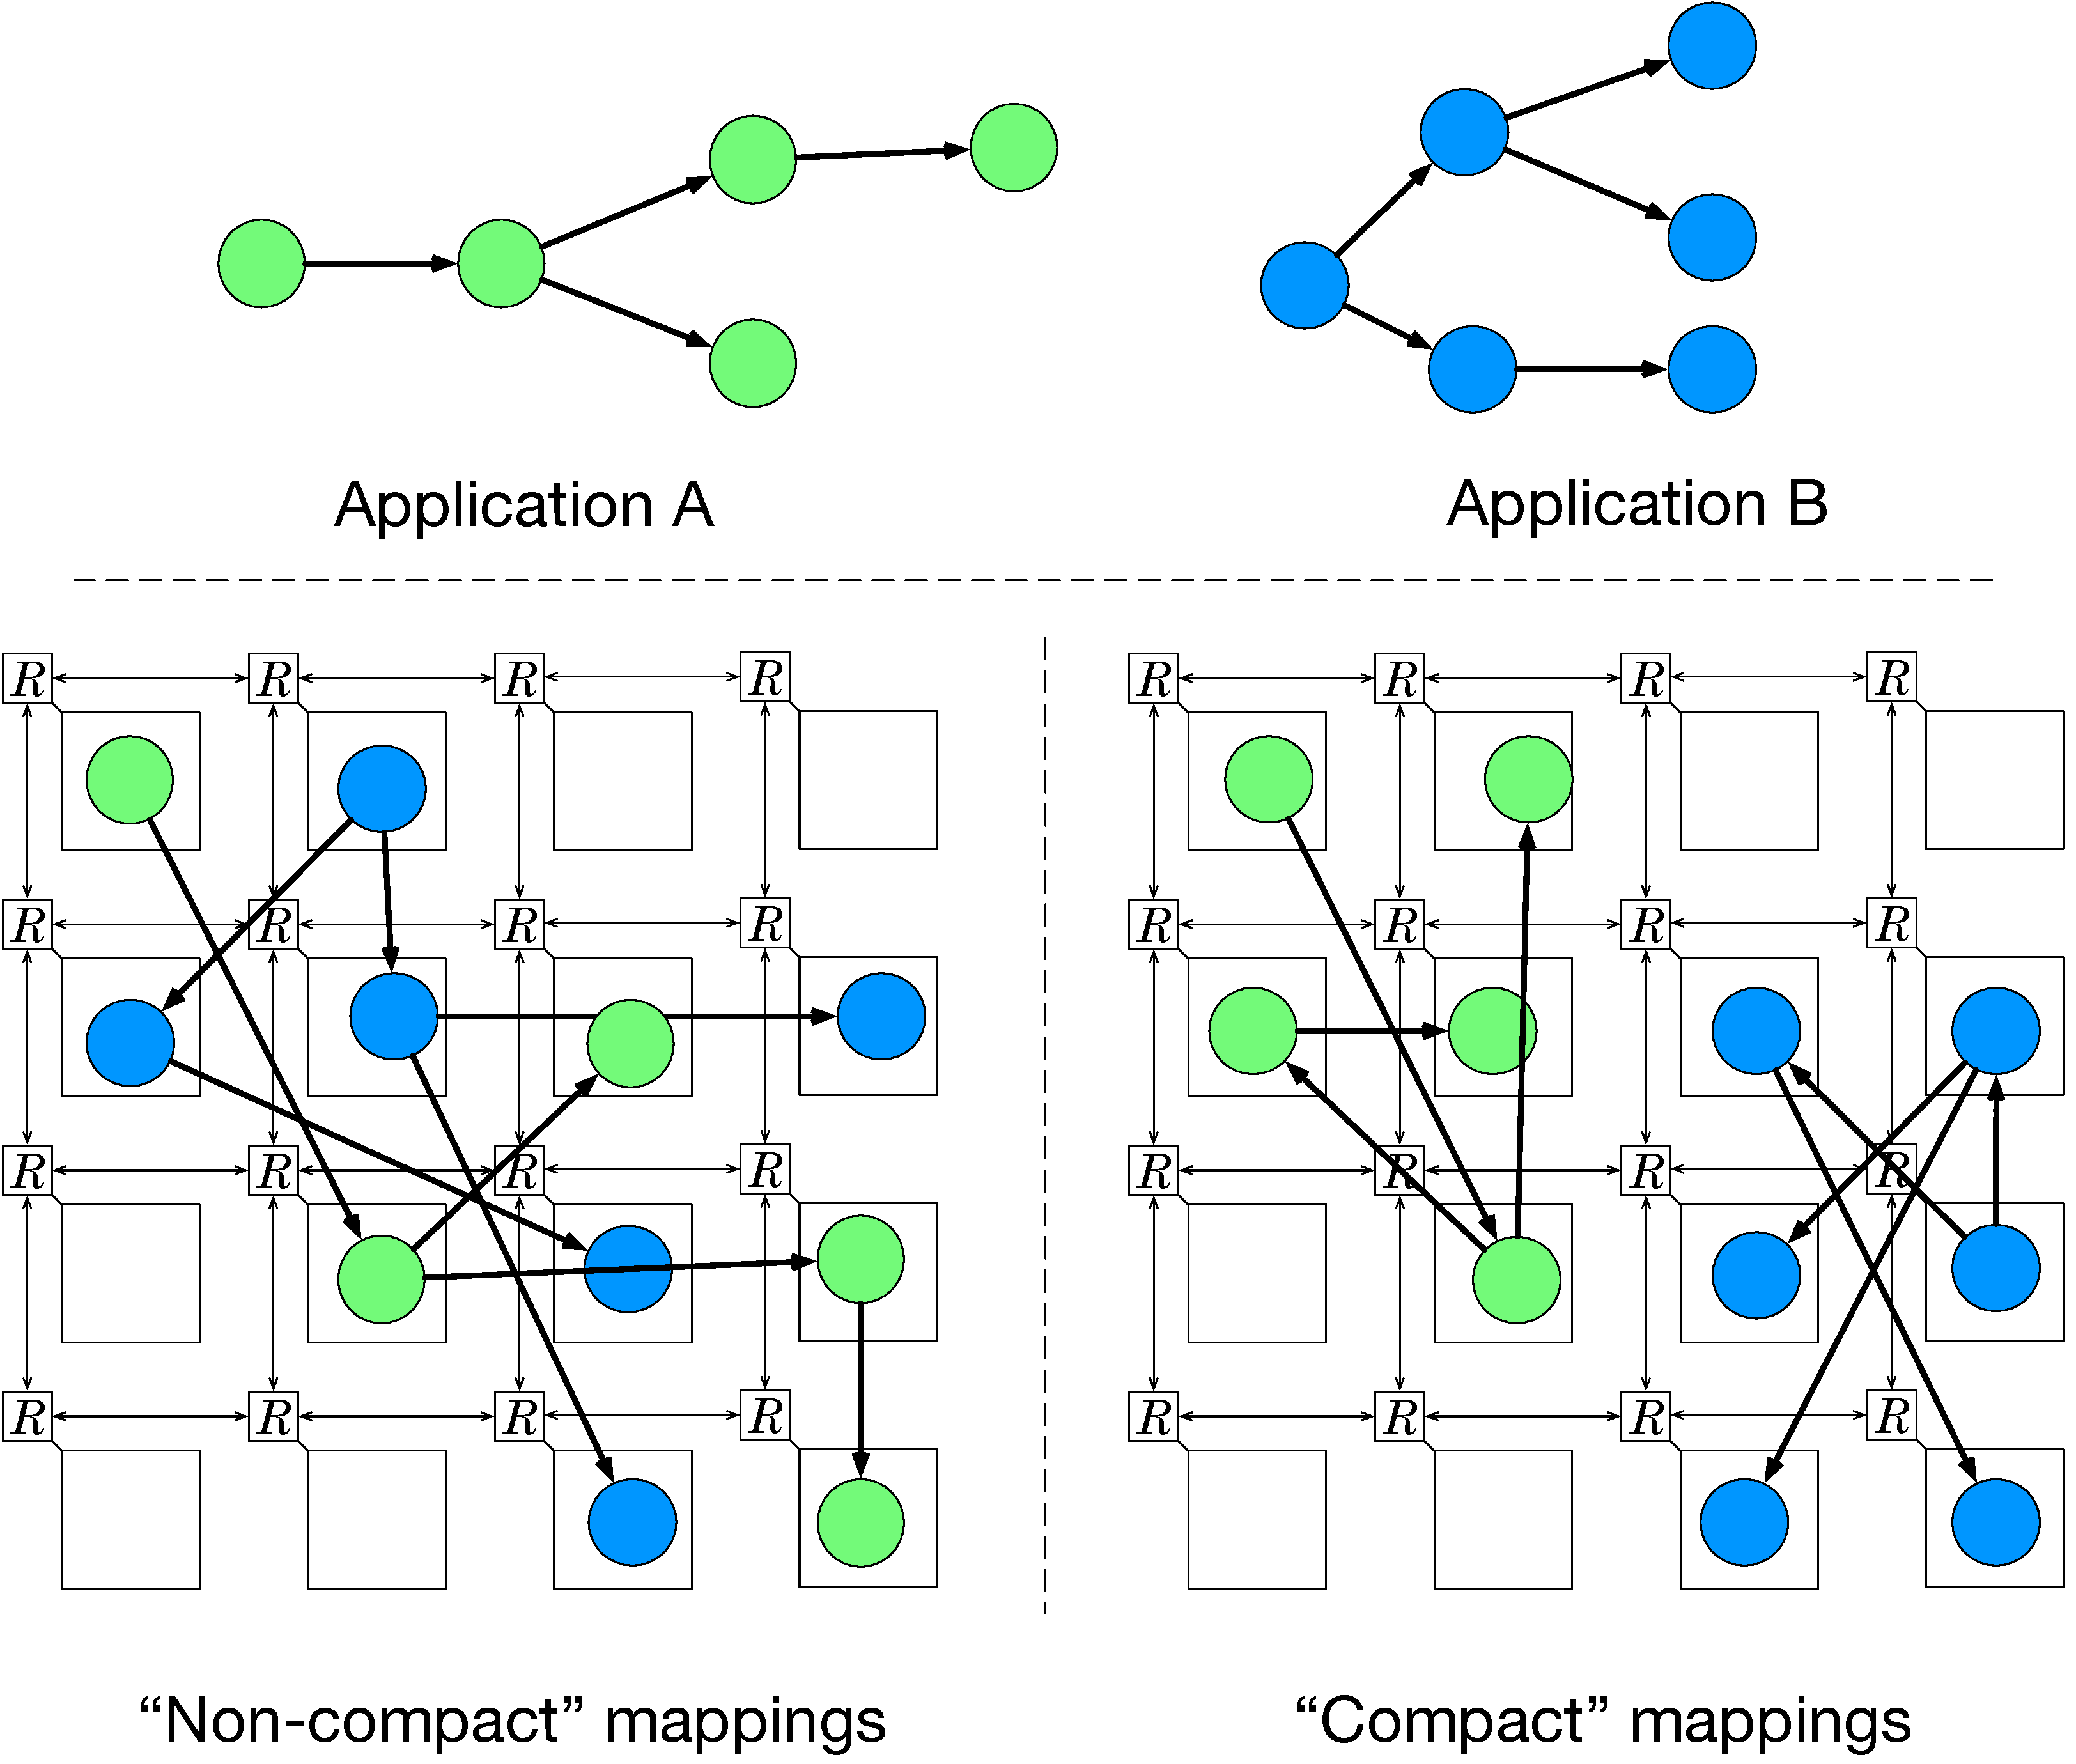
\includegraphics[width=0.6\textwidth]{figures/compact_intro.pdf}
	\caption{Equivalent mappings of two applications, one being compact and the other one not. Adapted from Figure~1 in~\cite{goens_samos19}.}
	\label{fig:compact_intro}
\end{figure*}

Figure~\ref{fig:compact_intro} illustrates well the idea of compact mappings.
It depicts two variants for mapping the two application graphs depicted in the figure.
The particular property of these two variants is that they are equivalent from the point of view of the distances:
For any two connected nodes in one of the application graphs, the node distance in terms of number of hops between both nodes is identical in both mapping variants.
Intuitively, however, it the mappings on the right are preferable to those on the left. 

Idea behind compact mappings, and why it does not work. Basically:\cite{goens_samos19}

\begin{figure*}[th]
	\centering
	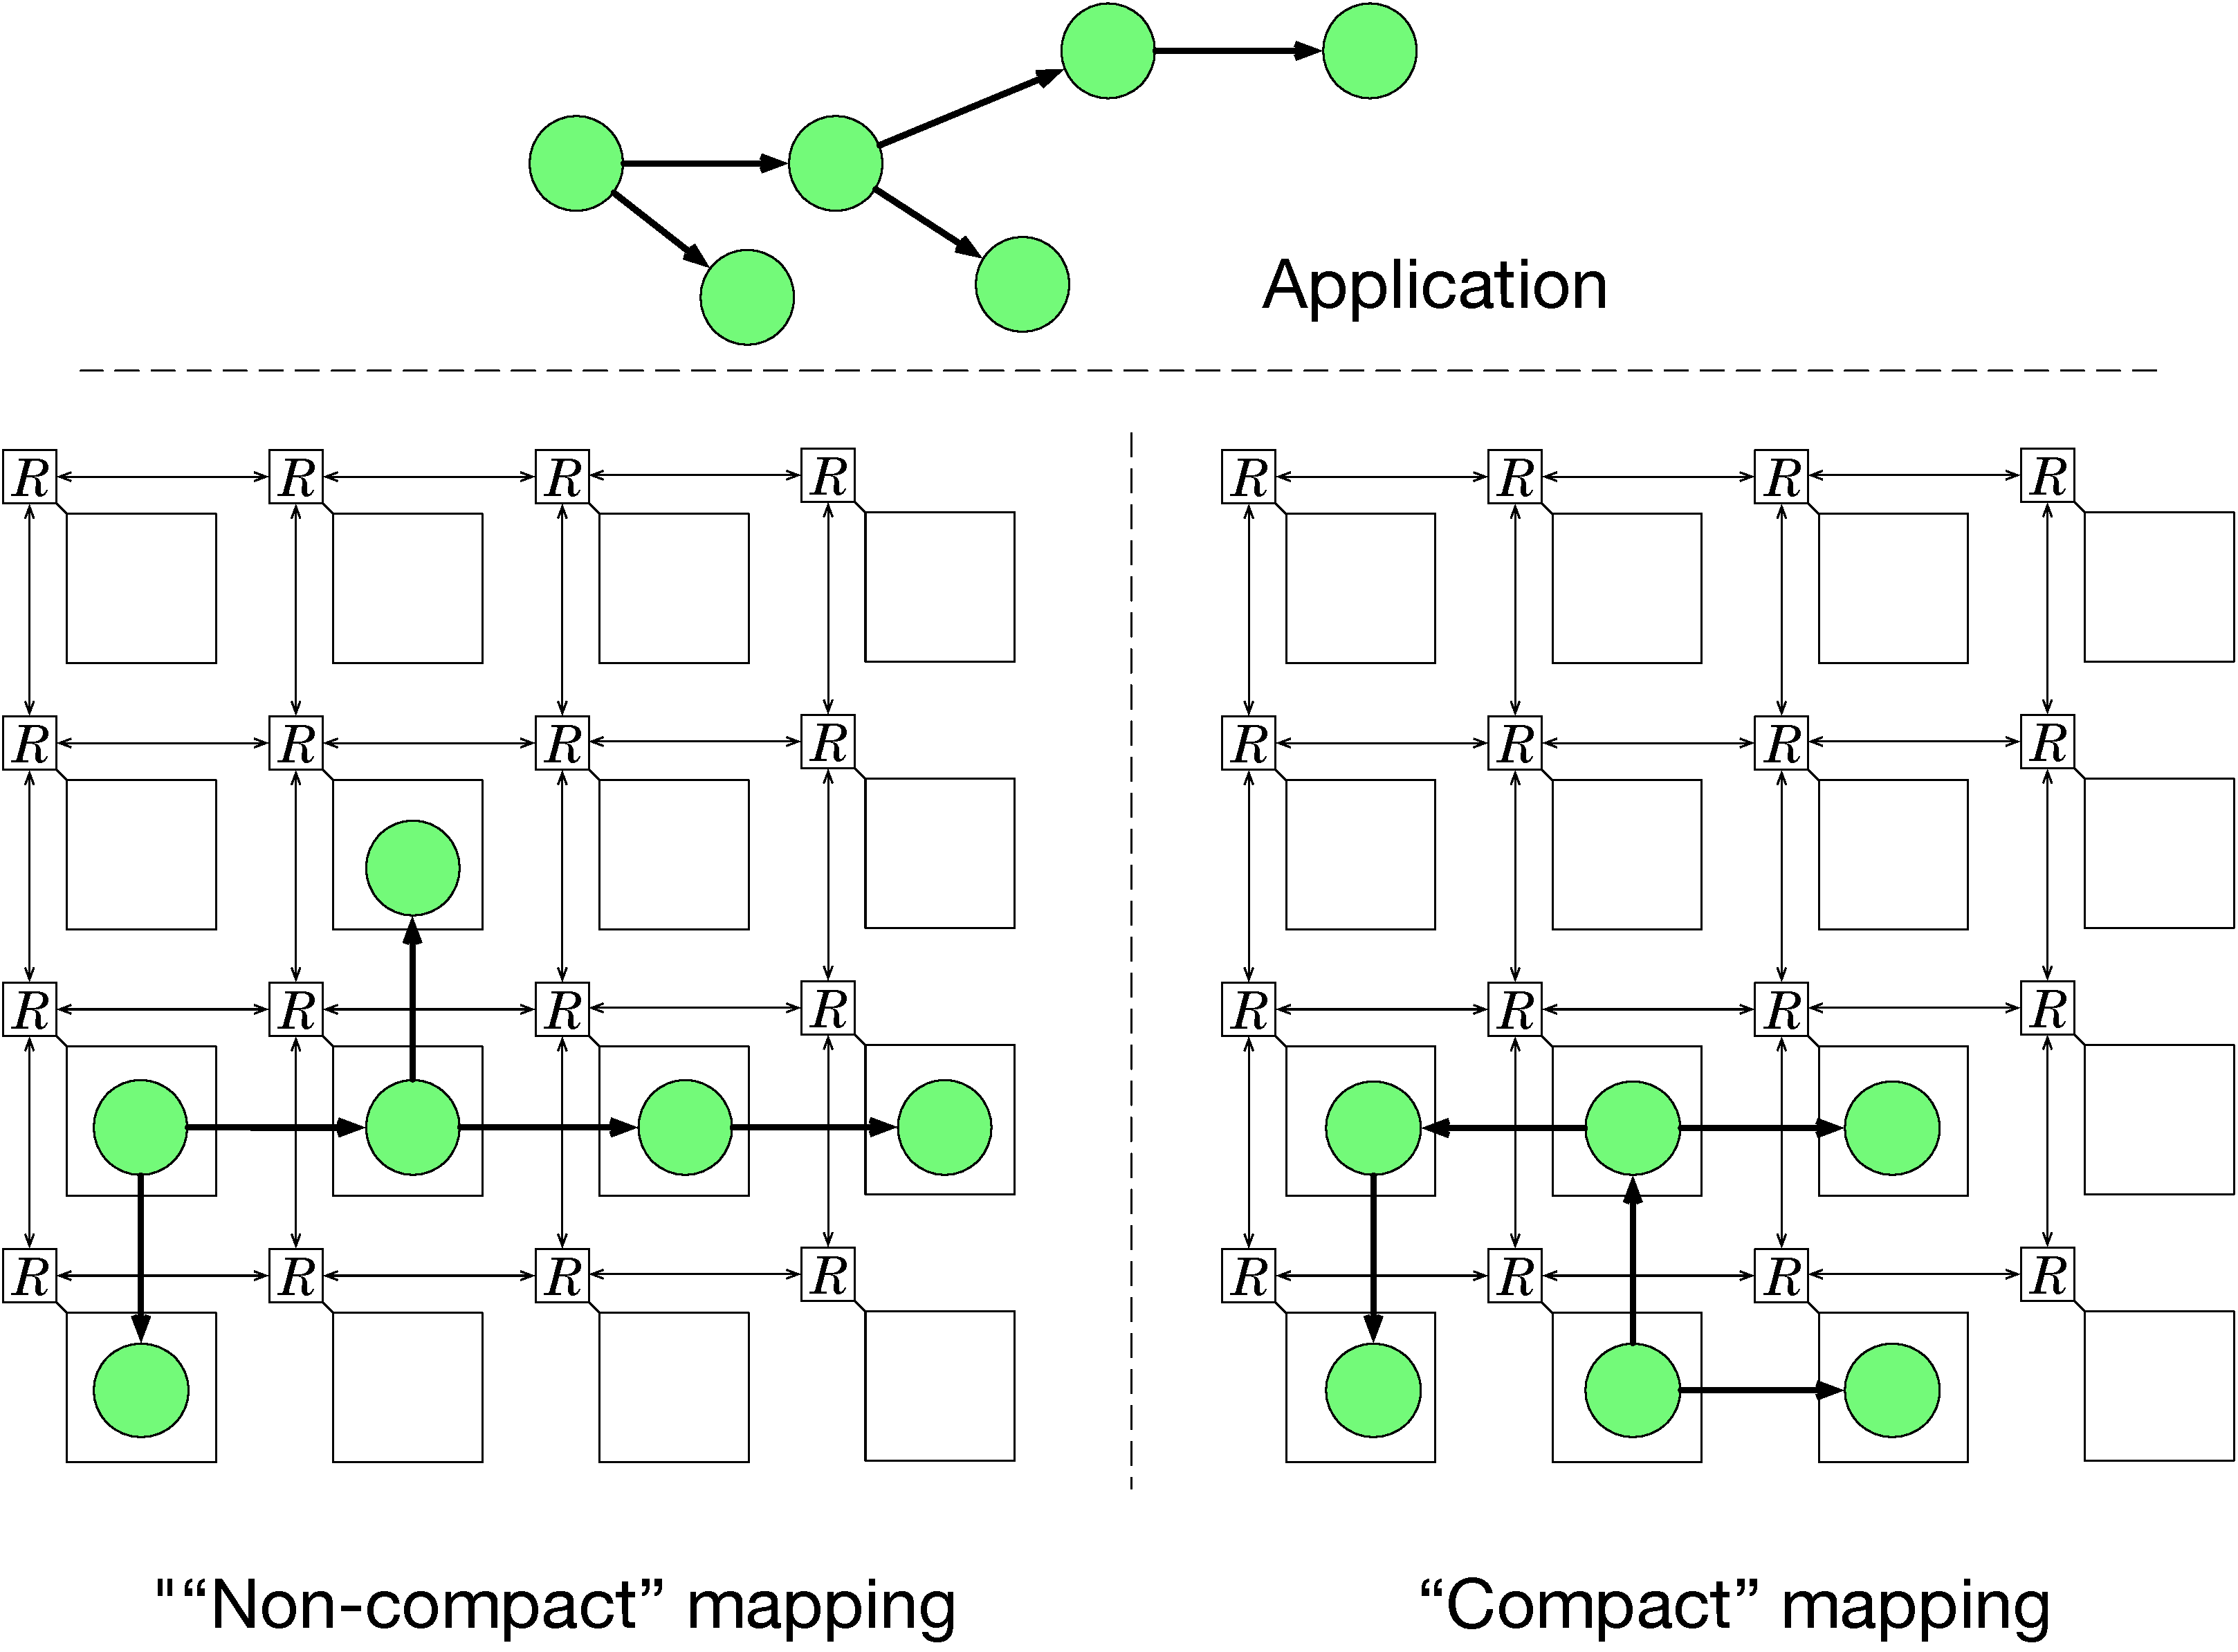
\includegraphics[width=0.6\textwidth]{figures/topology_vs_geometry.pdf}
	\caption{Two equivalent mappings that yield good performance. Adapted from Figure~2 in~\cite{goens_samos19}.}
	\label{fig:topology_vs_geometry}
\end{figure*}


\begin{figure}[h]
	\centering
   \resizebox{0.85\textwidth}{!}{\inputTikz{compact_latency.tex}}
	\caption{Comparison of latencies between compact, non-compact and random mappings. Adapted from Figure~4 in~\cite{goens_samos19}.}
	\label{fig:compact_latency}
\end{figure}


\begin{figure}[h]
	\centering
   \resizebox{0.85\textwidth}{!}{\inputTikz{compact_cases.tex}}
	\caption{Comparison between compact, non-compact and random mappings running isolation or with another 9 applications. Adapted from Figure~5 in~\cite{goens_samos19}.}
	\label{fig:compact_cases}
\end{figure}